\documentclass[varwidth=9.7cm]{standalone}
\usepackage{pgfplots}
\pgfplotsset{compat=1.18}
\usepgfplotslibrary{statistics,groupplots}
\usepgflibrary{plotmarks, patterns}
\usetikzlibrary{calc, patterns, shapes}
\usepackage{xcolor}
\usepackage{pifont}
\newcommand{\cmark}{\ding{51}}  
\newcommand{\xmark}{\ding{55}}

\definecolor{ibm1}{HTML}{0077BB}
\definecolor{ibm2}{HTML}{33BBEE}
\definecolor{ibm3}{HTML}{EE7733}
\definecolor{ibm4}{HTML}{EE3377}
\definecolor{ibm5}{HTML}{CC3311}

\definecolor{grad1}{HTML}{364B9A}
\definecolor{grad2}{HTML}{98CAE1}
\definecolor{grad3}{HTML}{FEDA8B}
\definecolor{grad4}{HTML}{DD3D2D}
\definecolor{grad5}{HTML}{A50026}


\begin{document}

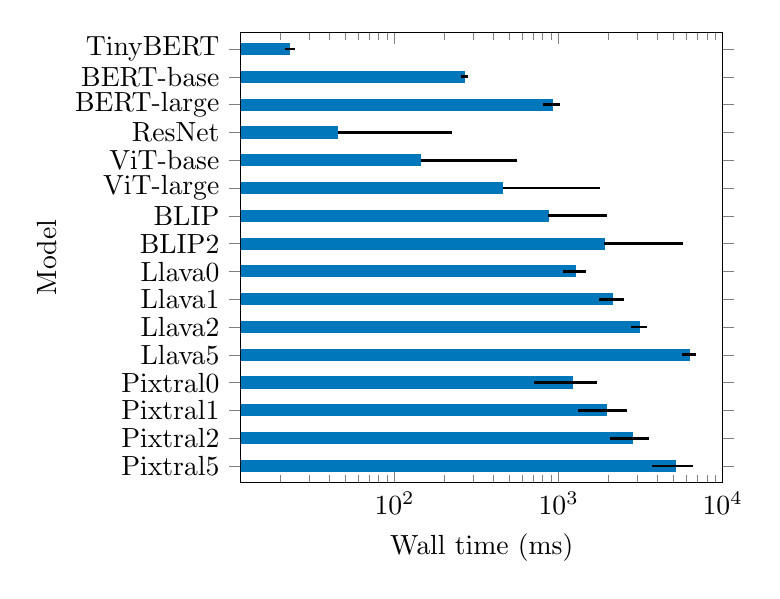
\begin{tikzpicture}

    \begin{axis}[
        xbar,
        xlabel={Wall time (ms)},
        ylabel={Model},
        symbolic y coords={
            Pixtral5,
            Pixtral2,
            Pixtral1,
            Pixtral0,
            Llava5,
            Llava2,
            Llava1,
            Llava0,
            BLIP2, BLIP, ViT-large, ViT-base, ResNet, BERT-large, BERT-base, TinyBERT,
            },
        ytick=data,
        width=7.7cm,
        enlarge y limits=0.04,
        height=7.3cm,
        bar width=4pt,
        xmax=10000,
        xmode=log,
        error bars/x dir=both,
        error bars/x explicit,
        error bars/error bar style={black, line width=1pt}, 
        error bars/error mark options={line width=1pt, mark size=0pt},
        set layers,
    ]
        \addplot+ [
            ibm1, 
            error bars/.cd, 
            x dir=both, 
            x explicit,
        ] coordinates {
            (23,TinyBERT) +- (1.6,0)
            (267,BERT-base) +- (14.7,0)
            (911,BERT-large) +- (111,0)
            (45,ResNet) +- (179,0)
            (144,ViT-base) +- (415,0)
            (455,ViT-large) +- (1320,0)
            (862,BLIP) +- (1107,0)
            (1900,BLIP2) +- (3794,0)
            (1269,Llava0) +- (200,0)
            (2127,Llava1) +- (362,0)
            (3119,Llava2) +- (344,0)
            (6243,Llava5) +- (594,0)
            (1215,Pixtral0) +- (506,0)
            (1967,Pixtral1) +- (648,0)
            (2802,Pixtral2) +- (759,0)
            (5165,Pixtral5) +- (1452,0)
        };
    \end{axis}

\end{tikzpicture}

\end{document}
